\label{sec:report_hardware_th}

Für die Umsetzung wurden handelsübliche Funksteckdosen verwendet, da diese relativ günstig in den meisten Geschäften zu haben sind. Diese erfüllen jedoch standardmäßig einen anderen Zweck, sie werden über eine Fernbedienung ein- bzw. ausgeschaltet. Da es uns nicht möglich ist, Steckdosen mit dem Raspberry über Funk zu steuern, musste eine andere Möglichkeit gefunden werden.\\
Uns kam die Idee, dass in diesen Steckdosen eigentlich nur ein Relais vorhanden sein muss, welches die 230V schaltet. Diese Tatsache machten wir uns zu nutze und suchten auf der Platine nach diesem Schaltpunkt und entwickelten eine passende Schaltung, welche diese Relais schaltet.\\\\
Um widerrechtliches Steuern der Steckdosen durch gefinkelte Schüler zu verhindern und da das Funkmodul nur auf die Platine aufgelötet war, bauten wir dieses aus. Somit ist es nicht mehr möglich die Steckdosen mit der passenden Fernbedienung zu steuern.\\\\
Die Schaltung der Steckdose ist in keinster Weise dokumentiert, auch die auf der Schaltung vorhandenen ICs sind kaum bis gar nicht dokumentiert, weshalb es uns nicht möglich war die Funktionsweise der einzelnen Teile festzustellen. Durch Analysieren der Leiterbahnen konnten wir uns eine grobe Übersicht über die Schaltung verschaffen. Dieser Überblick reichte jedoch nicht aus, um den Schaltpunkt des Relais zu finden. Der eigentliche Schaltpin am Relais konnte identifiziert werden, jedoch schaltet dieses Relais erst bei 48V, welche nicht vom Raspberry zur Verfügung gestellt werden, deshalb musste eine andere Möglichkeit gefunden werden.\\
Die Art des Suchens war nicht sehr professionell, da wir versuchten, durch Anlegen einer Steuerspannung an bestimmte Pins der ICs, den Pin zu finden, durch welchen das Relais geschaltet wird. Nach einigen Versuchen konnte der Punkt gefunden werden, dieser war jedoch nicht ideal, da dessen Innenwiderstand sehr klein war, was sich dahingehend zeigte, dass der Strom, der benötigt wurde, um die Steuerspannung zu halten, sehr hoch war. Wir fanden allerdings einen besseren Punkt, welcher wesentlich weniger Strom zog. (siehe \autoref{fig:report_hardware_plBo} Punkt 6) Durch das Anlegen von 5V schaltete das Relais, dies entspricht der Versorgungsspannung des Funkmoduls. Es liegt nahe, diese zu verwenden. (siehe \autoref{fig:report_hardware_plBo} Punkt 3)\\\\
Für eine leichtere Montage wurden die vorhandenen Kontakte des Funkmoduls verwendet (siehe \autoref{fig:report_hardware_plBo} Punkt 3 und 5). Über die Kontakte wurde die Platine versorgt, diese Funktionsweise verwendeten auch wir, weshalb wir von dem gefundenen Punkt eine Drahtbrücke zum Kontakt machten. Die 5V waren sowieso schon auf einem der Kontakte vorhanden. Um die ursprüngliche Funktion des anderen Kontaktes abzuschalten, trennten wir, durch Entfernen eines Widerstandes, (siehe \autoref{fig:report_hardware_plBo} Punkt 2) die Leiterbahn auf. Den gefunden Pin verbinden wir mit einer Drahtbrücke mit dem Kontakt. (siehe \autoref{fig:report_hardware_plBo} Punkt 4) Nun musste nur mehr die Platine in die Kontaktlöcher gesteckt werden. (siehe \autoref{fig:report_hardware_plTo} Punkt 1) Die nötigen Signale sind bei den Kontakten angelegt und werden über die Verbindung auf der Platine bereitgestellt.\\
Nun musste noch eine Lösung gefunden werden, wie diese 2 Punkte mit dem Raspberry Pi verbunden werden konnten. Dies wurde mit einer Transistorschaltung realisiert. Wenn der Raspberry an einem der GPIO-Pins digital 1 (analog 3,3V DC) anlegt, so schaltet der Transistor und verbindet somit die zwei Punkte. \\
Dies war jedoch nicht genug, da noch eine Potentialtrennung zwischen Raspberry und Steckdose  notwendig war, wie ein Test ohne Potentialtrennung zeigt. (siehe \autoref{sec:report_hardware_pot}). Diese lösten wir mit einem Optokoppler, welcher den Raspberry von der Steckdose trennen soll. Dies erfolgte mit der Schaltung ordnungsgemäß. Jedoch packten wir die Potentialtrennung auf den Header, welcher auf den Raspberry aufgesteckt wird, dies stellte sich als fataler Fehler heraus. (siehe \autoref{sec:report_hardware_spannung})\\
Der finale Aufbau war dann wie folgt:\\
Auf die GPIO-Pins (siehe \autoref{fig:report_hardware_gpio1}) wird eine Platine (Header) gesteckt (siehe \autoref{fig:report_hardware_heTo}), welche die Transistorschaltung beinhaltet. Diese Schaltung erfüllt den Zweck, die 5 V Versorgungsspannung auf den Eingang des Optokopplers zu bringen, welcher auf einer Platine in der Steckdose liegt. Die Verbindung wurde mit einem zweipoligen Draht, welcher auf beiden Seiten eine 3,5mm-Mono-Klinke-Stecker montiert hat, auf den beiden Endstücke wurden die dementsprechenden Buchsen montiert. (siehe \autoref{fig:report_hardware_heTo} Punkt 1 und \autoref{fig:report_hardware_plTo} Punkt 2) Auf der Platine in der Steckdose ist nur der Optokoppler (siehe \autoref{fig:report_hardware_plTo} Punkt 1), der das Ein- bzw. Ausschalten der Steckdose vornimmt.\\\\
Für die Kommunikation mit dem Raspberry wird der GPIO Pin 4 (Header Pin 7) verwendet. Die 5V Spannung und die Masse für das Schalten des Optokopplers wird der Pin 2 (5V) und der Pin 6 (0V) des Raspberrys verwendet. Wichtig: Hier ist anzumerken, dass die Rasperrys Revision 1 und Revision 2 verschiedene Pin-Anordnungen haben. Unsere Schaltung ist für Revision 2 entwickelt, es ist also nicht zu empfehlen, die Platine auf einem Revision 1 Raspberry zu verwenden, da er Schaden nehmen könnte.
\\
\begin{figure}[H]
\centering
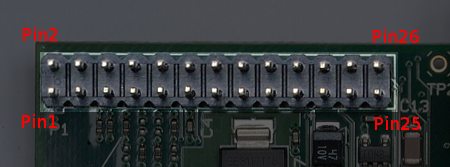
\includegraphics[keepaspectratio=true, width=10cm]{images/rpi/picPins.png}
\caption[GPIO-Pins]{GPIO-Pins\\ \textbf{Quelle:}  http://elinux.org/Rpi\_Low-level\_peripherals}
\label{fig:report_hardware_gpio1}
% source: http://elinux.org/Rpi_Low-level_peripherals#General_Purpose_Input.2FOutput_.28GPIO.29
\end{figure}
\begin{figure}[H]
\centering
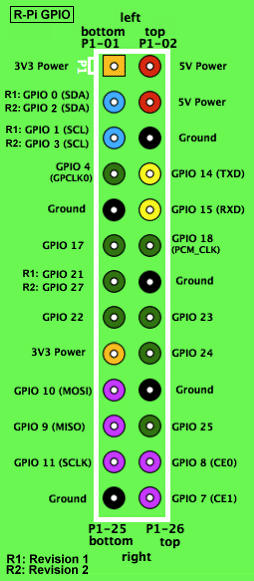
\includegraphics[keepaspectratio=true, width=6cm]{images/rpi/gpio.png}
% source: http://elinux.org/Rpi_Low-level_peripherals#General_Purpose_Input.2FOutput_.28GPIO.29
\caption[GPIO-Pinbelegung]{GPIO-Pinbelegung\\ \textbf{Quelle:} http://elinux.org/Rpi\_Low-level\_peripherals}
\label{fig:report_hardware_gpio2} 
\end{figure}
\begin{figure}[H]
\centering
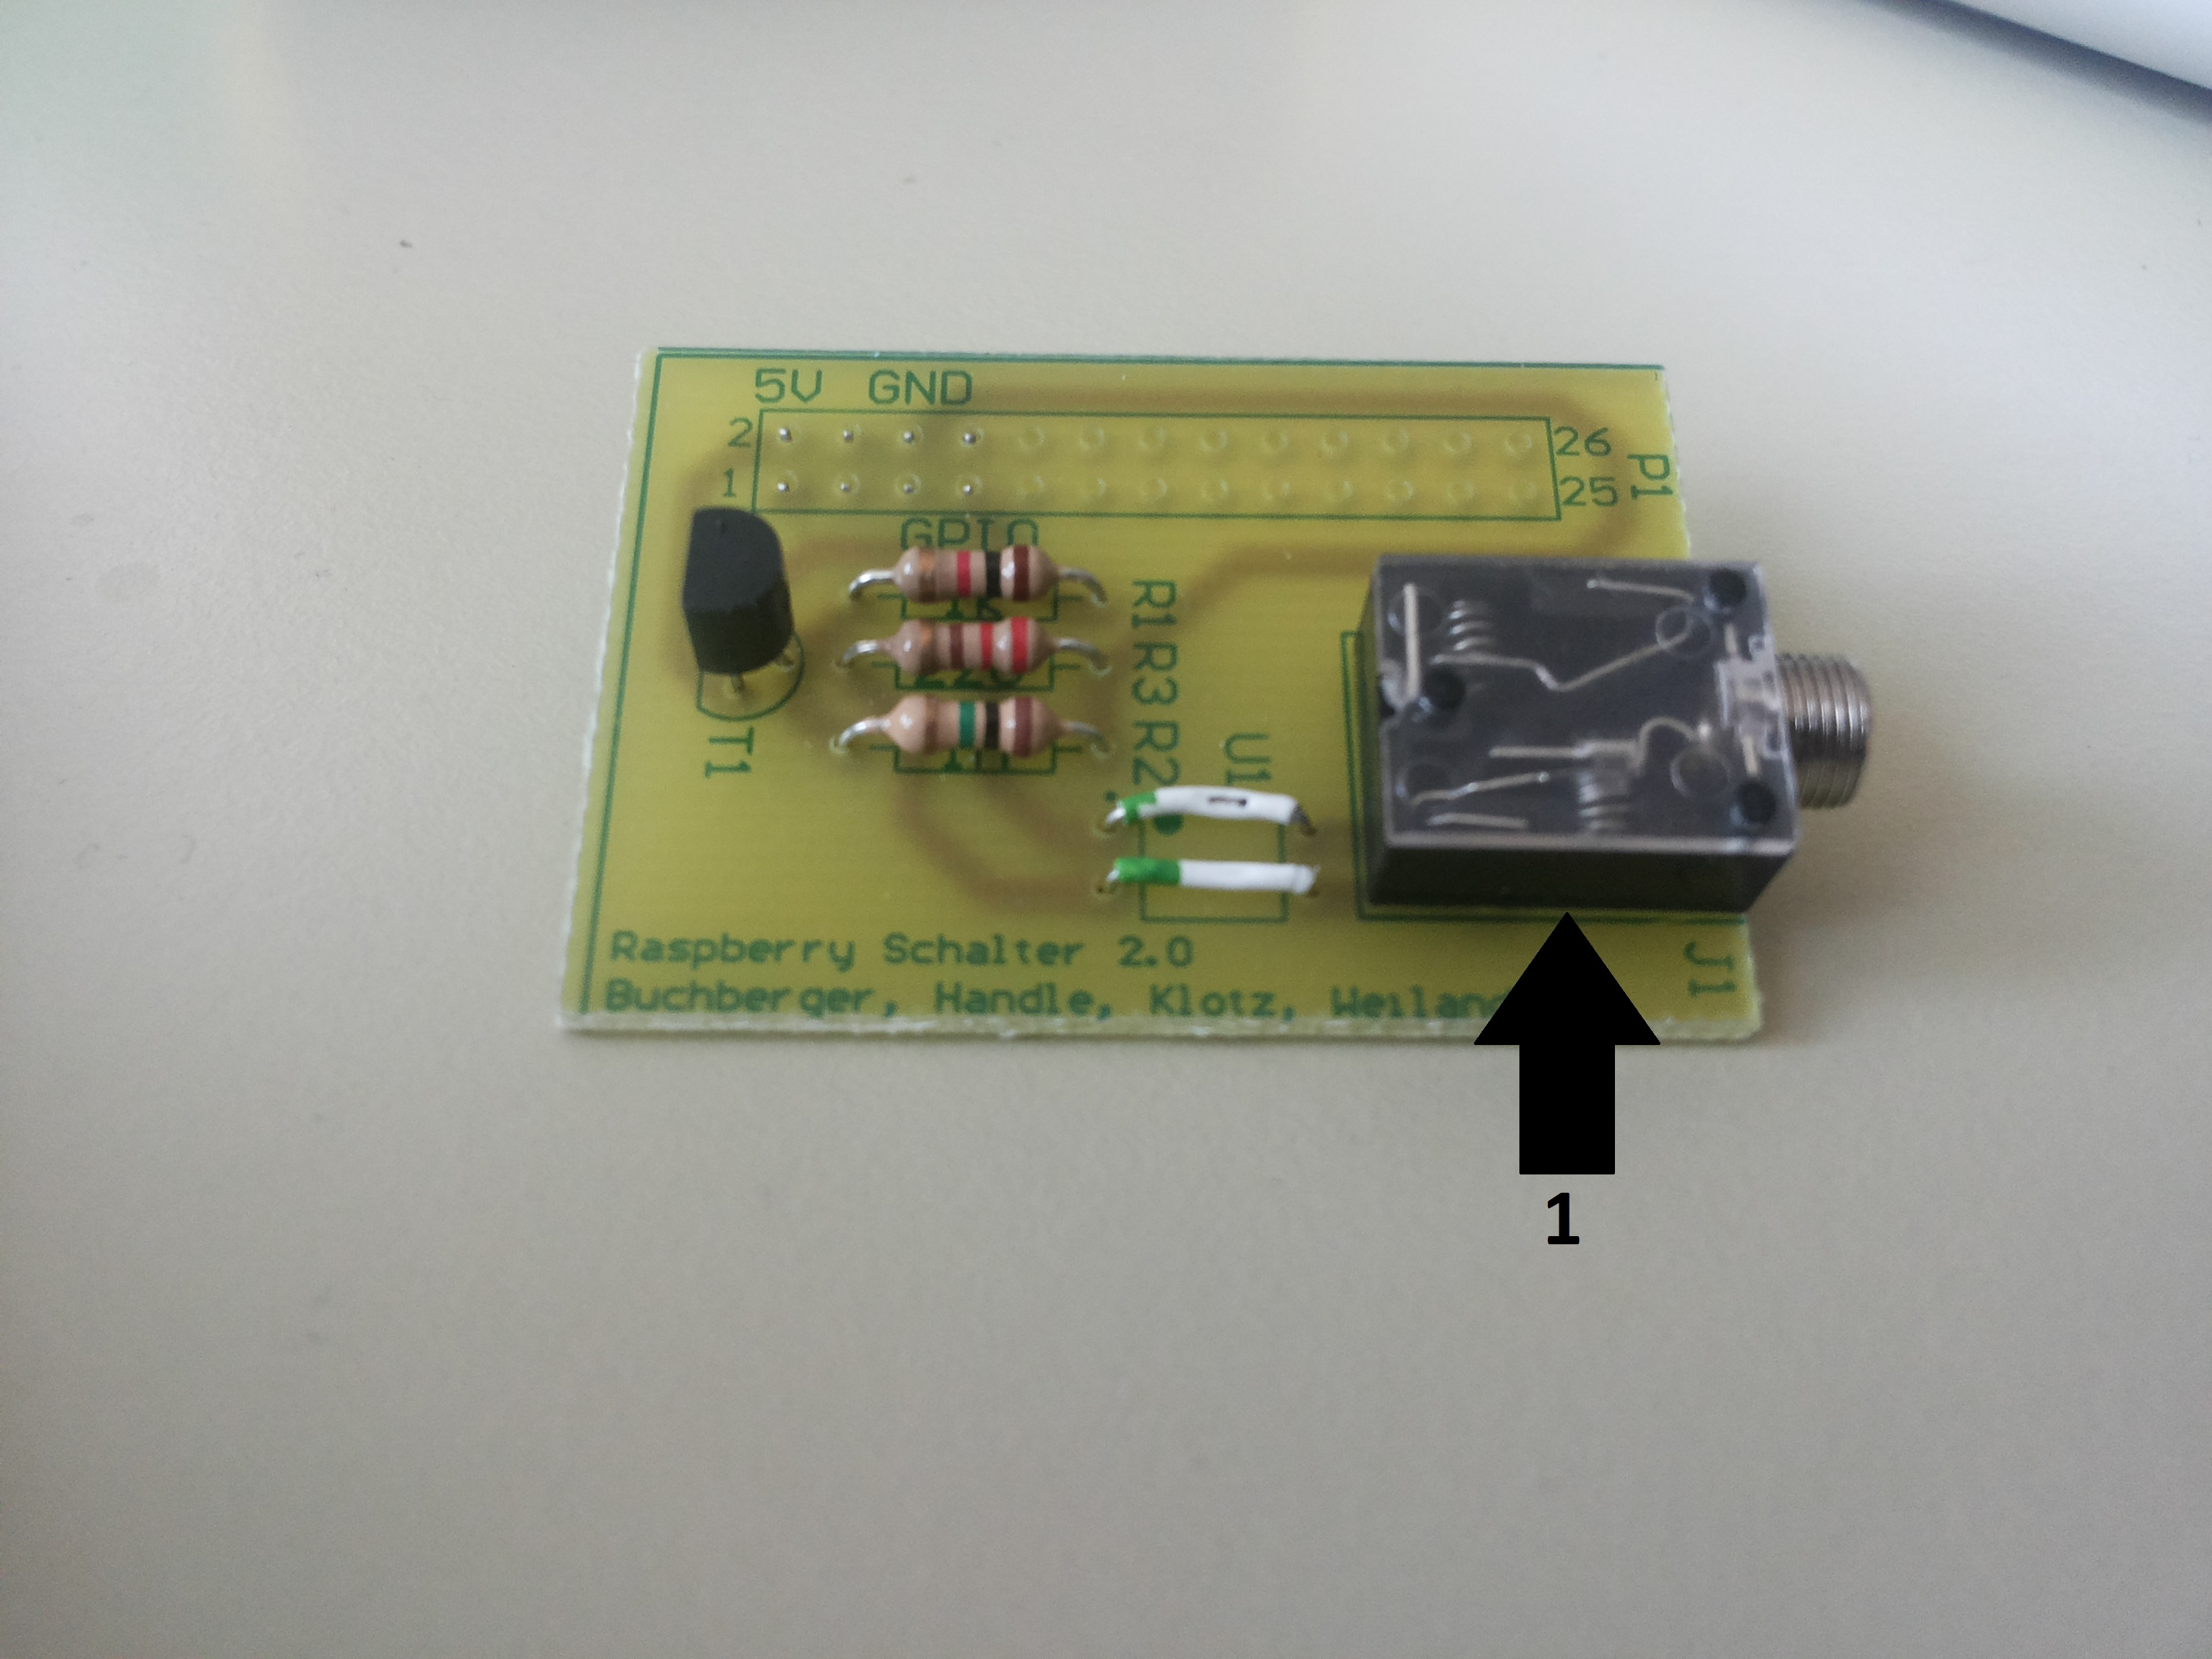
\includegraphics[keepaspectratio=true, width=13cm]{images/rpi/rpi_header_top.jpg}
\caption{Header oben}
\label{fig:report_hardware_heTo}
\end{figure}
\begin{figure}[H]
\centering
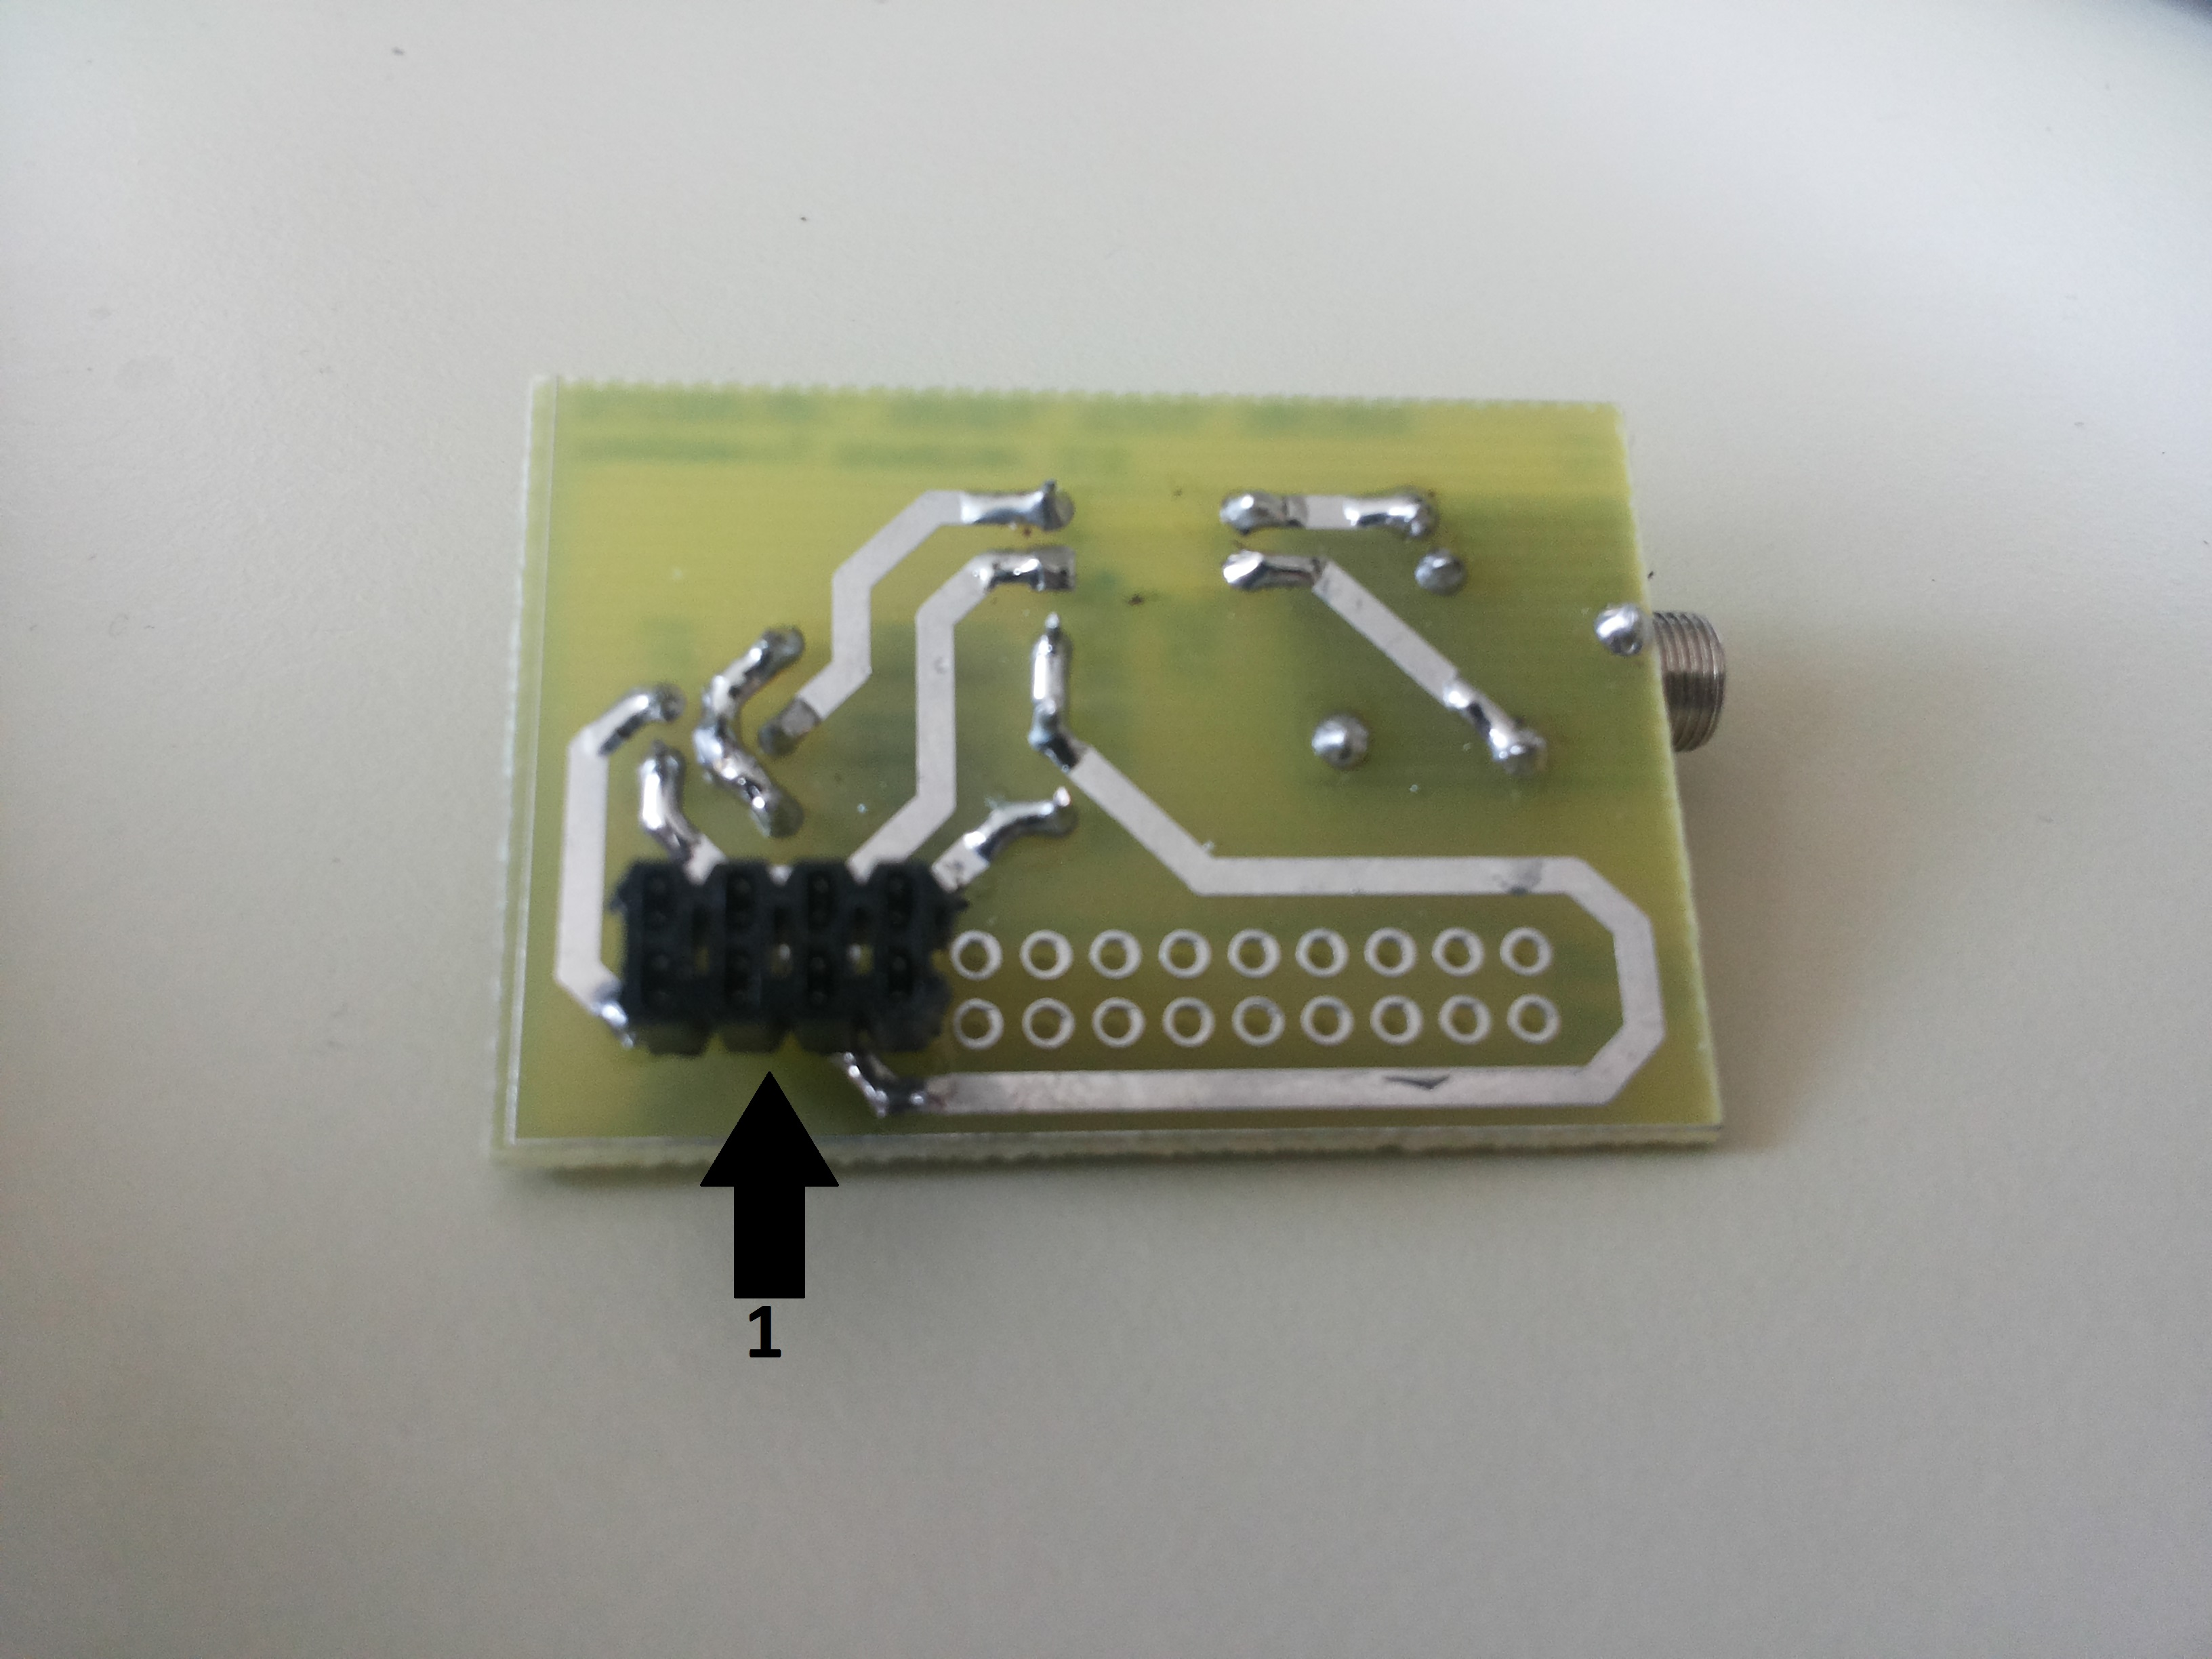
\includegraphics[keepaspectratio=true, width=13cm]{images/rpi/rpi_header_bottom.jpg}
\caption{Header unten}
\label{fig:report_hardware_heBo}
\end{figure}
\begin{figure}[H]
\centering
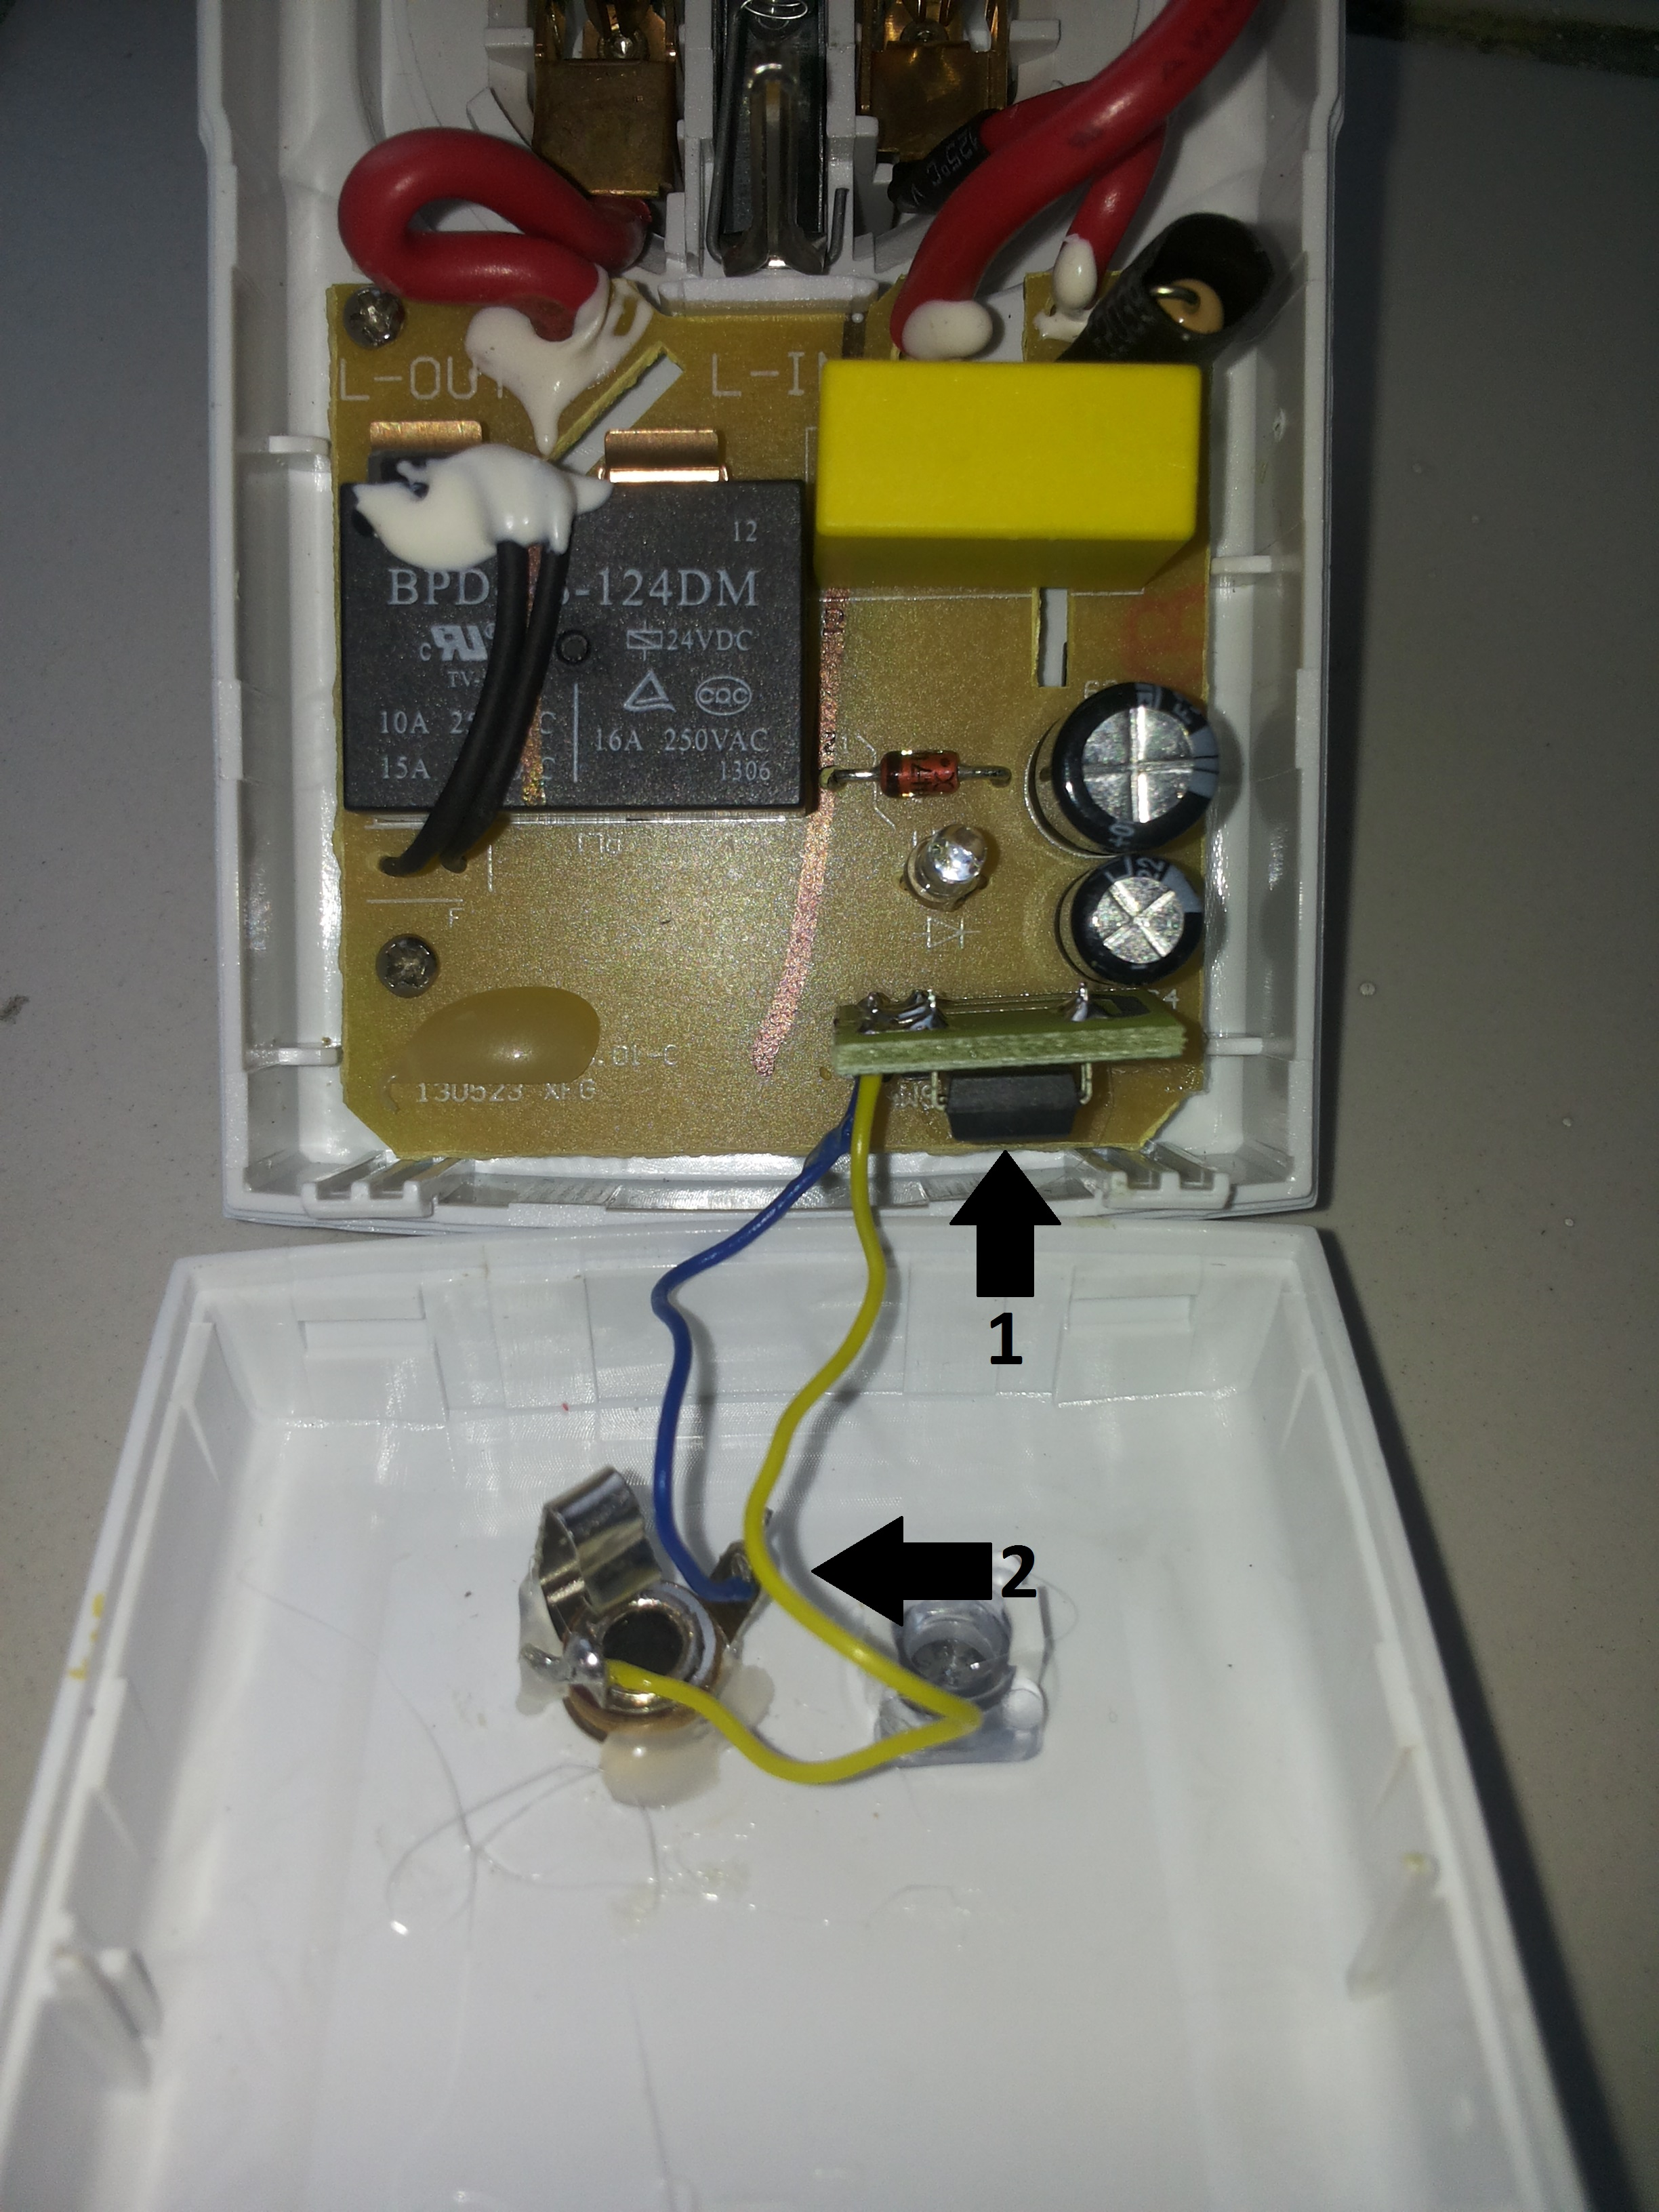
\includegraphics[keepaspectratio=true, width=13cm]{images/rpi/rpi_platine_top.jpg}
\caption{Steckdose offen}
\label{fig:report_hardware_plTo}
\end{figure}
\begin{figure}[H]
\centering
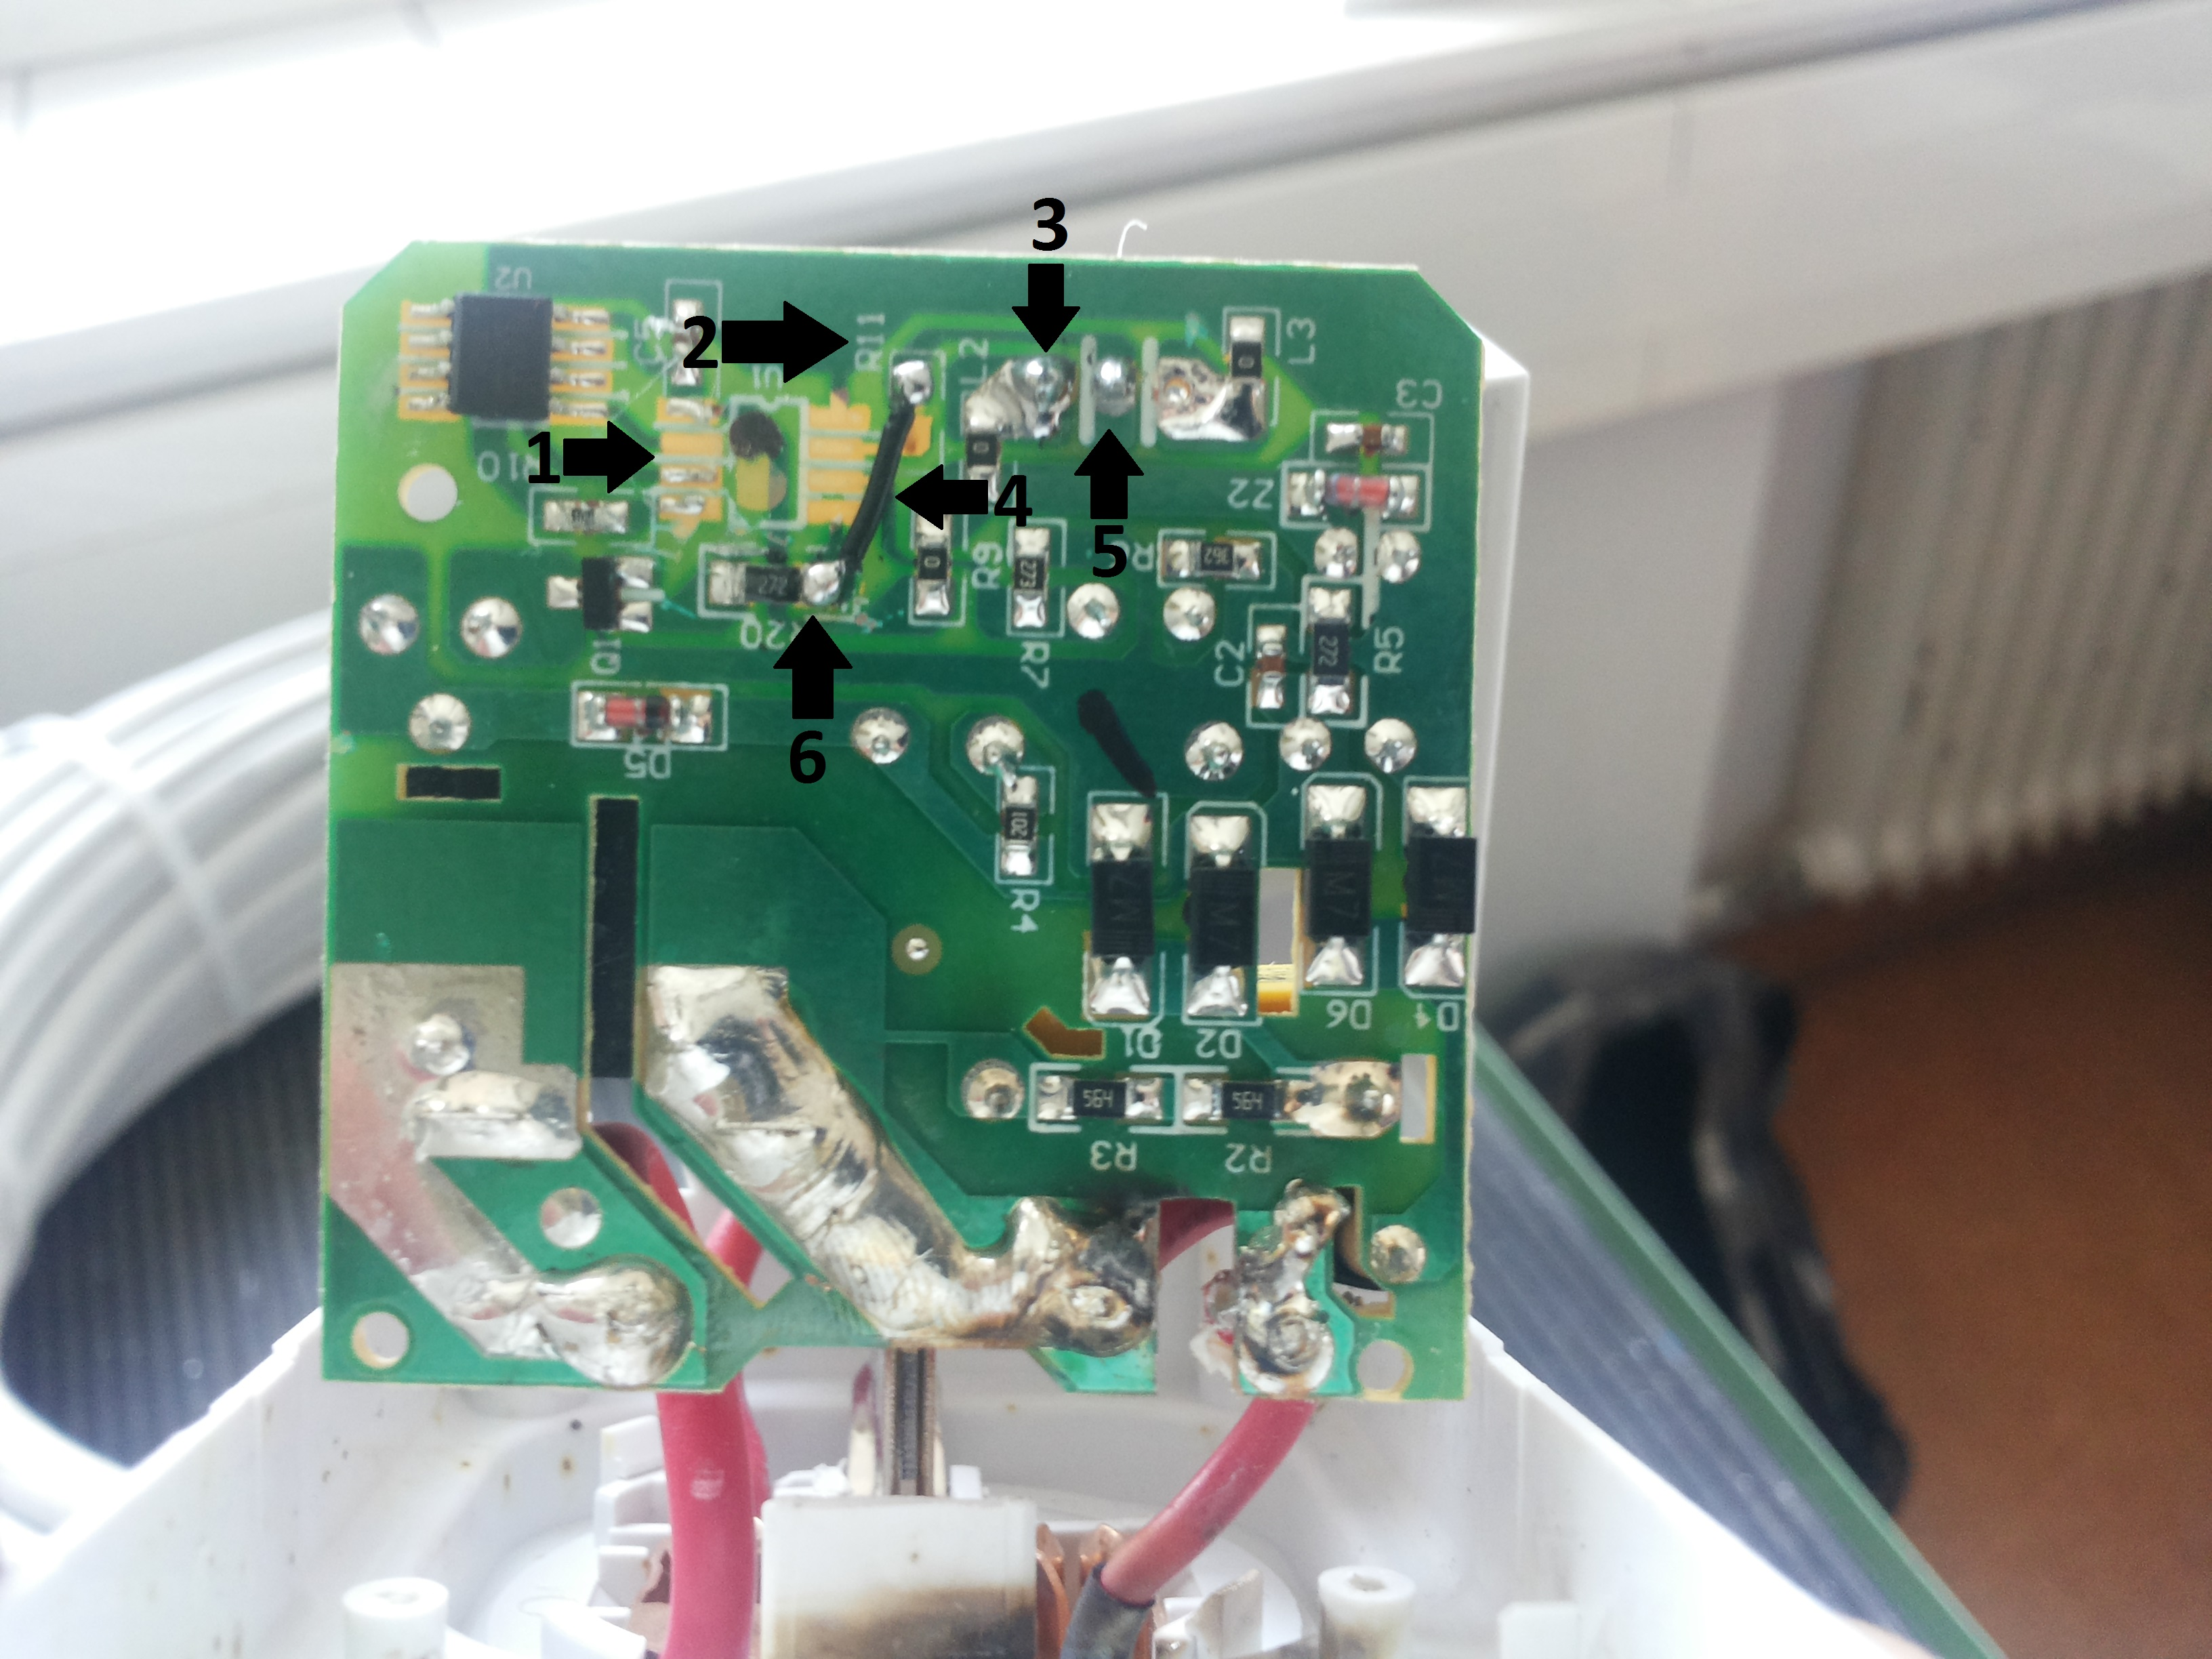
\includegraphics[keepaspectratio=true, width=17cm]{images/rpi/rpi_platine_bottom.jpg}
\caption{Platine unten}
\label{fig:report_hardware_plBo}
\end{figure}
\paragraph{Transistorplatine}
Diese Platine verbindet die Masse und die 5V des Raspberrys über einen Vorwiederstand kurz, wenn der Raspberry beim entsprechenden GPIO-Pin 1 anlegt. In der kurzgeschlossenen Leitung hängt die primäre Seite des Optokopplers.\\
\begin{figure}[H]
\centering
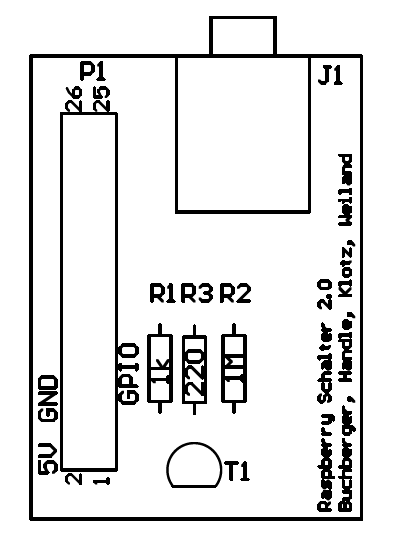
\includegraphics[keepaspectratio=true, height=6cm]{images/rpi/Transistorschaltung_Bestueckung.png}
\caption{Transistorschaltung Bestückung}
\label{fig:report_hardware_TransBest}
\end{figure}
\begin{figure}[H]
	\centering
	\begin{minipage}{7cm}
		\centering
		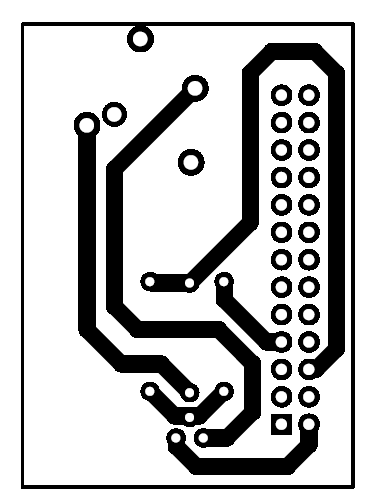
\includegraphics[keepaspectratio=true, height=6cm]{images/rpi/Transistorschaltung_BottomLayer.png}
		\caption{Transistorschaltung Bottom Layer}
		\label{fig:report_hardware_TransBL}
	\end{minipage}
	\hspace{1cm}
	\begin{minipage}{7cm}
		\centering
		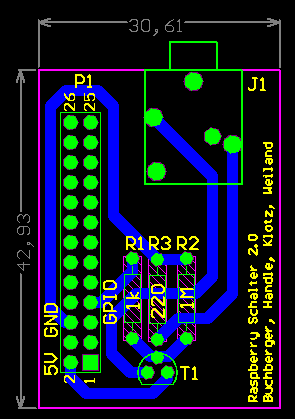
\includegraphics[keepaspectratio=true, height=6cm]{images/rpi/Transistorschaltung_PCB.png}
		\caption{Transistorschaltung PCB}
		\label{fig:report_hardware_TransPCB}
	\end{minipage}
\end{figure}
\begin{figure}[H]
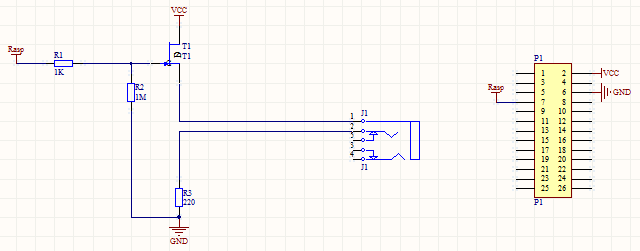
\includegraphics[keepaspectratio=true, width=17cm]{images/rpi/Transistorschaltung_Schematic.png}
\caption{Transistorschaltung Shematic}
\label{fig:report_hardware_TransSche}
\end{figure}
\paragraph{Optokopplerplatine}
Auf dieser Platine ist nur der Optokoppler. Die Leitungen die von der Transistorplatine am Optokoppler angeschlossen werden, werden an der Primärseite angeschlossen. Fließt hier genug Strom, so leuchtet die LED im Optokoppler und der interne Phototransistor leitet. Nun verbindet der Phototransistor die 2 Punkte, wie oben schon erwähnt und das Relais schaltet.\\
\begin{figure}[H]
\centering
	\begin{minipage}{7cm}
		\centering
		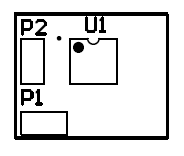
\includegraphics[keepaspectratio=true, height=4cm]{images/rpi/Optokoppler_Bestueckung.png}
		\caption{Optokoppler Bestückung}
		\label{fig:report_hardware_OptBest}
	\end{minipage}
	\hspace{1cm}
	\begin{minipage}{7cm}
		\centering
		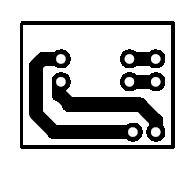
\includegraphics[keepaspectratio=true, height=4cm]{images/rpi/Optokoppler_BottomLayer.png}
		\caption{Optokoppler Bottom Layer}
		\label{fig:report_hardware_OptBL}
	\end{minipage}
\end{figure}
\begin{figure}[H]
\centering
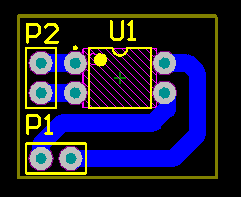
\includegraphics[keepaspectratio=true, height=4cm]{images/rpi/Optokoppler_PCB.png}
\caption{Optokoppler PCB}
\label{fig:report_hardware_OptPCB}
\end{figure}
\begin{figure}[H]
\centering
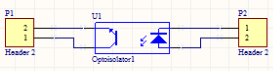
\includegraphics[keepaspectratio=true, width=10cm]{images/rpi/Optokoppler_Schematic.png}
\caption{Optokoppler Shematic}
\label{fig:report_hardware_OptSche}
\end{figure}

\subsection{Aufbau}

Siehe SIS-Administor-Anleitung unter Abschnitt Monitore.